\documentclass[12pt]{article}
\usepackage{gensymb}
\usepackage{amsmath}
\usepackage{graphics}
\usepackage{graphicx}
\graphicspath{{storage/self/primary/Download/asgnt5/fig}}
\graphicspath{{storage/self/primary/Download/asgnt5/table}}
\let\vec\mathbf
\usepackage{float}
\providecommand{\brak}[1]{\ensuremath{\left(#1\right)}}
\providecommand{\myvec}[1]{\ensuremath{\begin{pmatrix}#1\end{pmatrix}}}
\providecommand{\norm}[1]{\ensuremath{\lvert|#1\rvert|}}
\begin{document}
\title{\textbf{9.10.5.3}}
\date{}
\maketitle
\textbf{Question :} In  ,$\angle PQR = 100\degree$,where $P,Q$ and $R$ are points on a circle with centre $O$.Find $\angle OPR$.

\textbf{Solution :}
\begin{table}[H]
    \centering
       \begin{tabular}{|c|c|c|}
    \hline
    \textbf{Input Parameters} &\textbf{Description} &\textbf{Value} \\
    \hline
     $\vec{O}$& Center(at origin)&$\vec{0}$\\
     \hline
 $r$ & Radius &1\\
 \hline
 $\theta$&-&$100\degree$\\
 \hline
 $\alpha$&-&$165.4\degree$\\
 \hline
 $\beta$&-&$5\degree$\\
 \hline
  \end{tabular}

    \caption{Table of input parameters}
    \label{tab:tab:1}
\end{table}

\begin{table}[H]
    \centering
    \begin{tabular}{|c|c|c|}
    \hline
        \textbf{Output Parameters} &\textbf{Description} &\textbf{Value} \\
\hline
          $\vec{Q}$ & Point &$\myvec{\cos{\theta_1}\\\sin{\theta_1}}$\\
          \hline
          $\vec{P}$ & Point &$\myvec{\cos{\theta_2}\\\sin{\theta_2}}$ \\
         \hline
          $\vec{R}$ & Point &$\myvec{\cos{\theta_3}\\sin{\theta_3}}$ \\
         \hline
    \end{tabular}


    \caption{Table of output parameters}
    \label{tab:tab:2}
\end{table}
For getting the value of the $\angle OPR$
\begin{align}
    \cos{\angle OPR }&= \frac{\vec{\brak{O-P}}^{\top}\vec{\brak{R-P}}}{\vec{\norm{O-P}\norm{R-P}}}\\
	&=\sqrt{\frac{1-\cos{\brak{\theta_2-\theta_3}}}{2}}\\
	\angle OPR &= 10\degree
  \end{align}

  \begin{figure}[H]                                 
	  \centering                          
	  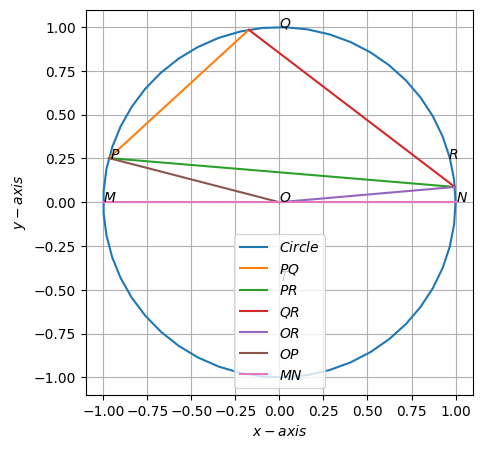
\includegraphics[width=\columnwidth]{fig/9.10.5.3.png}
\caption{}
\label{9.10.5.3}                        
  \end{figure}

\end{document}

